%نام و نام خانوادگی:
%شماره دانشجویی: 
\مسئله{}
رایج است که روش \lr{Quality Function Deployment} را در مرحله استخراج نیازمندی‌ها استفاده می‌کنند.
\begin{enumerate}[a)]
	\item
این روش را تعریف کنید و خروجی‌های آن و همچنین نحوه به دست آمدن این خروجی‌ها را شرح دهید.
	
	\item
یکی از دام‌هایی که در استخراج نیازمندی‌ها برای تیم‌های نرم‌افزاری پیش می‌آید \lr{Requirement Creep} است. در مورد این دام تحقیق کنید و شرح دهید که چیست و چگونه می‌توان از آن اجتناب کرد. (۵ روش را ذکر کنید.)
\end{enumerate}

\پاسخ{
\begin{enumerate}[a)]
\item

\textbf{
تعریف روش \lr{Quality Function Deployment}\cite{geeksforgeeks}}

این روش که به اختصار QFD نامیده می‌شود، روند یا مجموعه ابزاری است که نیازمندی‌های مشتری را برای طراحان محصول مشخص کرده و این نیازمندی‌ها را در قالب ویژگی‌های مهندسی (\lr{Engineering Specifications}) و برنامه‌های پیاده‌سازی در می‌آورد. اصلی که در این روش بیشترین اهمیت را دارد برآورده شدن تمامی خواسته‌های مشتری در رابطه با محصول است. این روش ۴ گام اساسی دارد که عبارتند از:
\begin{itemize}
	\item برنامه‌ریزی محصول (\lr{Product Planning}) 
	
	در مرحله اول باید نیازمندی‌های مشتری به صورت مجموعه‌ای از نیازمندی‌هایِ طراحیِ اولویت‌بندی شده درآورده شود. محصولات رقیب و شناسایی تفاوت‌های آنها با محصول مورد نظر نیز در این مرحله انجام می‌شود. 
	
	\item برنامه‌ریزی قسمت‌ (\lr{Part Planning})
	
	در این بخش باید مشخص شود که به ازای هر نیازمندی مشتری، چه ویژگی‌هایی باید در محصول گنجانده شوند. برای مثال اگر هدف مشتری «رابط کاربری خوب» است، باید ویژگی‌های «طراحی زیبا» و «سهولت کارکرد» در لیست مشخصات قرار گیرند. 
	
	\item برنامه‌ریزی روند (\lr{Process Planning})

پس از مشخص شدن مشخصات محصول، باید روند موثر و کارآمدی برای پیاده‌سازی آنها پیدا شود.
	
	\item برنامه‌ریزی تولید (\lr{Production Planning})

در نهایت نیز پس از تعیین فرآيند، روند ساخت و ارائه محصول مورد بررسی قرار می‌گیرد.
\end{itemize}

با وجود آن‌که روش‌های QFD در تمامی مراحل ساخت نرم‌افزار مورد استفاده قرار می‌گیرند، تنها روش‌های ویژه‌ای از آن می‌توانند برای استخراج نیازمندی‌ها مورد استفاده قرار گیرند. در این روش‌های خاص از مصاحبه با مشتری‌ها و مشاهده، مطالعه و پژوهش‌ بر روی داده‌های پیشین برنامه به عنوان داده‌های خام برای جمع‌آوری نیازمندی‌ها استفاده می‌کنند. این داده‌ها پس از جمع‌آوری در داخل جدولی گنجانده می‌شوند که به آن «جدول صدای مشتری (\lr{Customer Voice Table})» نیز گفته می‌شود. با آماده شدن این جدول روش‌های مختلفی برای دسته‌بندی نیازمندی‌های مشتری اعمال می‌شوند (نیازمندی‌ها دارای انواع گوناگونی هستند که شامل \lr{Expected Requiements} و \lr{Exciting Requirements} هستند)\cite{swbook}.

\textbf{خروجی‌ها و نحوه محاسبه آنها}

یکی از مهم‌ترین ابزارهای مورد استفاده در روش \lr{QFD}، ابزار «خانه کیفیت (\lr{House of Quality})» است\cite{sixsigma}. با استفاده از این روش می‌توان تصمیم‌گیری آگاهانه‌تری در رابطه با نیازمندی‌های مشتریان انجام داد. این ابزار در واقع یک ماتریس است که رابطه بین نیازمندی‌های مشتری و توانایی محصول و سازنده در پاسخگویی به این نیازها را نشان می‌دهد. نمونه‌ای از این ماتریس و معرفی بخش‌های متخلف آن در ادامه آورده شده است.

\begin{figure}[h]
	\centering
	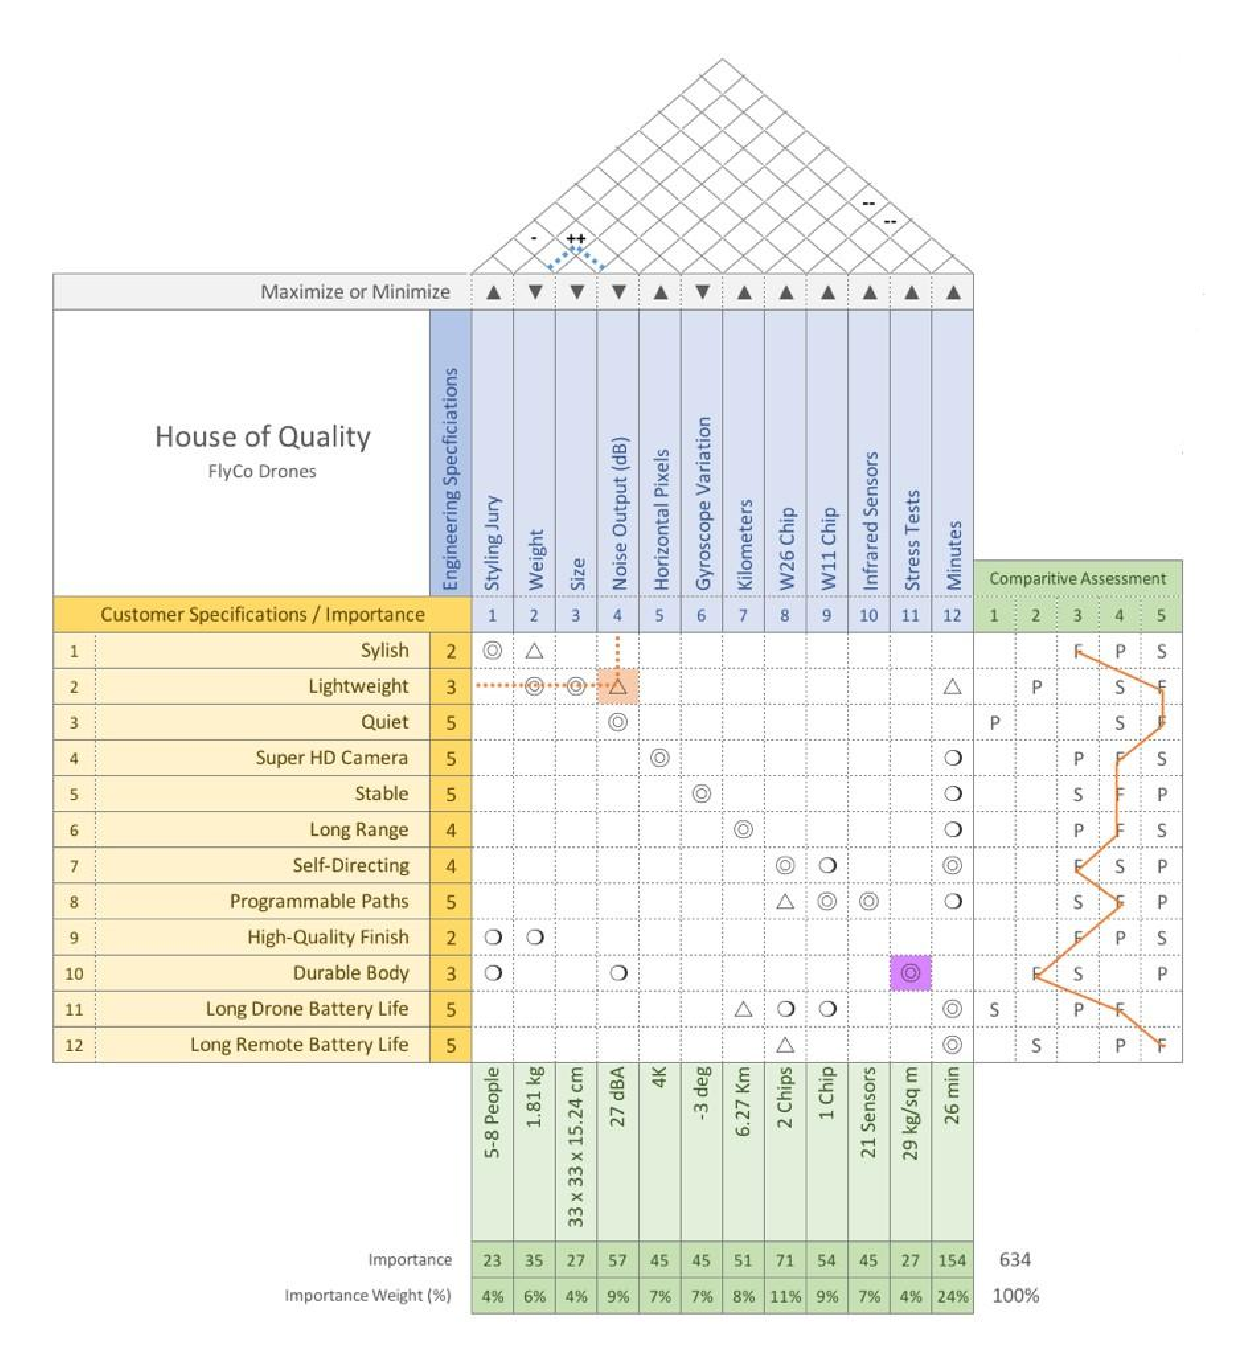
\includegraphics[scale=0.55]{figs/2-1.pdf}
	\caption{یک نمونه \lr{House of Quality}}
	\label{fig2}
\end{figure}

\begin{itemize}
\item
\lr{Customer Specification}: این بخش که در سمت چپ خانه قرار گرفته است، ویژگی‌های حائز اهمیت برای مشتری که بر روی آنها تمرکز زیادی دارد را نشان می‌دهد. اعدادی که در سمت راست این ستون و روبه‌روی هر ویژگی‌ نوشته شده است نشان‌دهنده میزان اهمیت آن در مقیاس ۱ تا ۵ است.

\item
\lr{Engineering Specification}: این بخش روش‌های مهندسی لازم برای اندازه‌گیری و پیش‌برد تولید را شامل می‌شود (ویژگی‌های قابل اندازه‌گیری برنامه). 

\item
\lr{Specific Measurements}: به ازای هر ویژگیِ نیازمندِ اندازه‌گیری که در بخش قبلی (\lr{Engineering Specification}) نوشته شده است، لازم است واحد اندازه‌گیری آن نیز تعیین شود. این بخش همان پایین‌ترین بخش است که با رنگ سبر مشخص شده است.

\item
\lr{Center Grid}: در بخش مرکزی میزان ارتباط بین هر ویژگی مد نظر مشتری و اندازه‌گیری‌های کمی مهندسی مشخص می‌شود. با توجه به راهنمای جدول که در شکل \ref{fig3} نشان داده شده است، $\circledcirc$ نشان‌دهنده ارتباط قوی با وزن ۹ است. شکل $\vartriangle$ رابطه متوسط با وزن ۳ را نشان می‌دهد و در نهایت شکل دایره نماینده وزن ۱ و رابطه ضعیف است.

برای مثال در شکل \ref{fig2}، نماد مثلث در رابطه بین \lr{Noise Output} و \lr{Lightweight} نشان‌دهنده آن است که بین میزان سنگینی محصول ساخته شده (در اینجا یک ربات) و میزان صدای تولید شده از آن رابطه متوسطی وجود دارد. 

\begin{figure}[h]
	\centering
	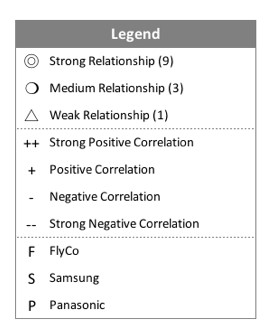
\includegraphics[scale=0.8]{figs/2-2}
	\caption{معرفی نمادهای استفاده شده در خانه کیفیت}
	\label{fig3}
\end{figure}

\item
\lr{Roof}: سقف خانه نشان‌دهنده تضادهای احتمالی بین کمیت‌های قابل‌اندازه‌گیری است. اگر خط نقطه‌چین شده آبی در شکل \ref{fig2} را دنبال کنیم، می‌بینیم که ارتباط مستقیم و قوی‌ای بین وزن و میزان صدای خروجی وجود دارد. در ردیف پایینی سقف نیز فلش‌های بالا و پایین نشان‌ می‌دهند که کمیت مورد نظر باید بیشینه شود یا کمینه. فلش رو به پایین برای اندازه نشان‌ می‌دهد که هر چقدر ابعاد محصول کوچکتر باشد به هدف مشتری نزدیکتر است. 

در بخش پایینی خانه که شامل واحد‌های اندازه‌گیری \lr{Engineering Specifications} است، دو سطر وجود دارد که در واقع سطرهای نهایی مورد نظر ما هستند. سطر اول نشان‌دهنده اهمیت تجمیعی کمیت است و سطر پایینی، میزان این اهمیت را بر حسب درصد مشخص می‌کند تا اهمیت نسبی مشخصه‌ها نسبت به یکدیگر نیز واضح‌تر شود. برای به دست آوردن importance کافیست میزان اهمیت \lr{Customer Specification} در وزن رابطه آن با مشخصه ضرب شده و تمامی مقادیر با هم جمع شوند. برای مثال در ویژگی \lr{Styling Jury}، \lr{Stylish} دارای اهمیت ۲، \lr{High-Quality Finish} دارای اهمیت ۲ و \lr{Durable Body} اهمیت ۳ را دارد. با توجه به علائم قرار گرفته در برابر هر کدام از این ويژگی‌ها در نهایت داریم:
\begin{latin}
$importance = 2\times 9 + 2 \times 1 + 3\times 1 = 23$
\end{latin}
پس از محاسبه تمامی مقادیر importance آنها را با هم جمع می‌کنیم تا به عدد نهایی \lr{634} برسیم. کافیست میزان اهمیت هر یک از مقادیر را بر این عدد نهایی تقسیم کنیم تا اهمیت درصدی را به دست آوریم. 
\end{itemize}

علاوه بر خروجی به دست آمده از خانه کیفیت که نشان‌دهنده میزان اهمیت هر ویژگی‌ است و با کمک آن می‌توان برخی مشخصه‌ها را حذف نمود، خروجی‌های دیگری نیز در نتیجه استخراج نیازمندی‌ها تولید می‌شوند\cite{swbook}. این خروجی‌ها که به اندازه پروژه وابسته هستند عبارتند از:

\begin{enumerate}
	\item معرفی نیازمندی‌ها و امکان‌سنجی آنها
	\item مشخص نمودن محدوده (scope) برنامه یا محصول
	\item لیستی از مشتری‌ها، کاربران و سایر ذی‌ینفعانی که در مرحله استخراج نیازمندی‌ها شرکت داشته‌اند
	\item توصیفی از محیط فنی سیستم 
	\item لیستی از تمامی نیازمندی‌های مطرح شده به همراه محدودیت‌های هر یک
	\item مجموعه‌ای از سناریوهای ممکن که در حین استفاده از محصول یا برنامه ممکن است اتفاق بیفتند
	\item نمونه‌های اولیه احتمالی تولید شده برای تعریف بهتر نیازمندی‌ها
\end{enumerate} 

\item

\textbf{معرفی \lr{Requirement Creep} و روش‌های اجتناب از آن}

\end{enumerate}

\subsection*{مراجع}

\begin{latin}
	\begingroup
	\renewcommand{\section}[2]{}%
	
\begin{thebibliography}{9}
%   Check this for adding items: https://www.student.unsw.edu.au/how-do-i-cite-electronic-sources
	

	\bibitem{geeksforgeeks}
	17, P. (2020, August 17),
	\textit{Quality function deployment (QFD) in software quality},
	Accessed on 12/5/2022, 
	\url{https://www.geeksforgeeks.org/quality-function-deployment-qfd-in-software-quality/}.

	\bibitem{swbook}
	Roger Pressman, Maxim, D., Pressman, R. S., \& Bruce R. Maxim, D. (2014),
	\textit{Software Engineering: A Practitioner’s Approach (Vol. 8)},
	McGraw-Hill Education.

	\bibitem{sixsigma}
	Six Sigma. (2022),
	\textit{What is house of Quality / QFD Example. What is Six Sigma? – Certification, Training, Lean},
	Accessed on 12/8/2022, 
	\url{https://www.whatissixsigma.net/house-of-quality-qfd/}.

\end{thebibliography}
\endgroup
\end{latin}

}
\newpage
